\documentclass[letterpaper, 10 pt, conference]{IEEEconf}
\usepackage[utf8]{inputenc}
\usepackage[T1]{fontenc}
\usepackage[style=ieee]{biblatex}
\usepackage{tikz}
\usetikzlibrary{positioning,fit,arrows.meta,backgrounds}
\usepackage{amsmath, amssymb, xcolor, tikz, pgfplots, pgfplotstable}

\newcommand{\todo}[1]{{\color{red}#1}}

\title{\LARGE \bf
A Pipeline to Assemble (Near-)Collision Footage Datasets
}

\author{
         Ben Upenieks, Chaitanya Varier,\\
         Curtis Duy Kha Phan, Jack David Roberts Williamson,\\
         Nicholas Geofroy, Tony Meng, Vincent-Olivier Roch\\
         University of Waterloo\\
         \\
         \tt\small ben.upenieks@uwaterloo.ca, cvarier@uwaterloo.ca,
         \\ \tt\small cdkphan@uwaterloo.ca, jdrwilli@uwaterloo.ca,
         \\ \tt\small nicholas.geofroy@uwaterloo.ca, c24meng@uwaterloo.ca, vroch@uwaterloo.ca
}

\bibliography{sources}
\begin{document}

\maketitle
\thispagestyle{empty}
\pagestyle{empty}


%%%%%%%%%%%%%%%%%%%%%%%%%%%%%%%%%%%%%%%%%%%%%%%%%%%%%%%%%%%%%%%%%%%%%%%%%%%%%%%%
\begin{abstract}

\todo{Write the abstract}

\end{abstract}

%%%%%%%%%%%%%%%%%%%%%%%%%%%%%%%%%%%%%%%%%%%%%%%%%%%%%%%%%%%%%%%%%%%%%%%%%%%%%%%%
\section{INTRODUCTION}

In the advent of connected vehicles and autonomous transportation, equipping consumer vehicles with the necessary equipment to facilitate high-end automated collision avoidance systems can be prohibitively expensive.
Technologies such as Radar, LIDAR and high-end cameras that are typically used for collision prediction are likely too expensive for most consumers and might not easily be affixed to their vehicles (maybe not true).
On the other hand dash-cams, cheap video cameras that can be mounted to a car's dashboard, have become increasingly affordable and prevalent as a means to capture a driver’s perspective.
Typically used for insurance purposes, dash-cams have the added benefit of recording a wide variety of collisions that wouldn't be feasible to simulate. 
This has led to the creation of many online communities to share videos of these rare situations on websites such as Reddit, Youtube, and Imgur.
We propose that this egocentric dash-cam video stream can be leveraged by computer vision systems to act as an affordable and commonplace sensor for automated collision prediction. 

In this paper we present a software pipeline to facilitate the collection, processing and annotation of egocentric dash-cam videos from various online video repositories to produce datasets that can be used to train deep dash-cam collision prediction models.
We aim to generate datasets that are not constrained to any regions or countries but rather provide location-agnostic data that is representative of general, global road and vehicle conditions.
These datasets will also be collision-oriented as the majority of these videos contain collisions for people's entertainment.
Current autonomous vehicle data collection techniques typically require astronomically expensive hardware and equipment and, consequently, are rarely involved in collisions and intentionally not put in high risk environments that may lead to a collision.
This is the data we hope to capture by taking advantage of existing videos of non-artificial collisions.

The pipeline uses web-scraping techniques to fetch the video data from these websites, along with a set of video metadata, describing the video's contents.
We use this data, in combination with the manually annotated data in order to create the collision dataset.
This combination allows us to take advantage of the wide variety of videos available on the internet, while still having reliable data that has been curated manually.
\todo{Not sure what else to put here}



%%%%%%%%%%%%%%%%%%%%%%%%%%%%%%%%%%%%%%%%%%%%%%%%%%%%%%%%%%%%%%%%%%%%%%%%%%%%%%%%
\section{RELATED WORK}

Chan et al.   \cite{chan2016anticipating}
approach the same problem of collision prediction via egocentric dash-cam videos. They propose a novel Dynamic-Spatial-Attention Recurrent Neural Network that distributes attention to localized and tracked vehicles within the video and models temporal dependencies to predict the earliest frame of a potential impending collision. Released with their paper is a dataset of 678 dash-cam videos capturing areas in Taiwan. Each video is annotated with vehicle tracking bounding boxes, the vehicles that were involved in the collision and the frame of the collision. We hope to allow researchers to expand on this dataset with location-agnostic data and similar annotations.



\subsection{Dash-cams}%
\label{sub:dash_cams}







%%%%%%%%%%%%%%%%%%%%%%%%%%%%%%%%%%%%%%%%%%%%%%%%%%%%%%%%%%%%%%%%%%%%%%%%%%%%%%%%
\section{METHODOLOGY}

\todo{Write the METHODOLOGY}
\begin{itemize}
  \item Major pipeline
  \item Presenting a graph or figure of the pipeline architecture
  \begin{itemize}
    \item pre-processing
    \item Tracking we can mention how prepare to solve the tracking problem (challenge and future work)
    \item Anonymization (tracking and blurring of vehicle plates and faces)
  \end{itemize}
\end{itemize}


\begin{figure}[htpb]
		\centering
    \tikzset{
        module/.style={%
            draw, rounded corners,
            minimum width=#1,
            minimum height=7mm,
            font=\sffamily
            },
        module/.default=2cm,
        >=LaTeX
    }
    \begin{tikzpicture}[
      % This will show the frame around the figure
      show background rectangle]

      % Place first 6 items
      \node[module] (crawler) {Web-Scrapers};
      \node[module, below=of crawler] (downloader) {Downloaders};
      \node[module, below=of downloader] (splitter) {Video-Splitter};
      \node[module, below=of splitter] (labeller) {Video-Labelling Tool};
      \node[module, below=of labeller] (face-blur) {Face Blurring};
      \node[module, below=of face-blur] (license-blur) {License Plate Blurring};
      \node[draw,inner xsep=4mm,inner ysep=7mm,fit=(face-blur)(license-blur)](anon){};
      \node[anchor=north west,inner sep=1pt] at (anon.north west) 
        {Anonymization};
      \node[module, below=of anon] (uploader) {Data-Uploader};
      \draw[->] (crawler)--(downloader);
      \draw[->] (downloader)--(splitter);
      \draw[->] (splitter)--(labeller);
      \draw[->] (labeller)--(face-blur);
      \draw[->] (face-blur)--(license-blur);
      \draw[->] (license-blur)--(uploader);

    \end{tikzpicture}
		\caption{Architecture of the default pipeline}
		\label{fig:obj-by-class}
\end{figure}


\subsection{Video Collection}


The entry into our pipeline is a set of web scraper executors that each target and scrape a specific website or video repository based on a user-defined set of key-terms, and an executor that pulls unlabelled videos from the user's database. Videos that are pulled by the scrapers are immediately added to the database with relevant metadata and marked as unlabelled. Subsequently, they are loaded into memory and sequentially fed into the pipeline. If the pipeline terminates before labelling a video, it remains flagged as unlabelled in the database and the video will be pulled in a subsequent run by the database source executor. Crawler state is maintained via database lookup of specified key-value pairs to ensure duplicate data is not pulled. No video preprocessing such as resizing, trimming or cropping is automatically performed.

Users may define their own search terms to be used when querying the video repository. This value can be set either in the crawler implementation (\todo{or the yaml pipeline configuration file?}). By default, our scrapers query using the keywords: (\todo{should probably define default keywords}). Currently we support scraping and querying Reddit, YouTube and Imgur. Users that want to pull from a video repository that is not currently implemented should create a custom executor and implement the \texttt{iCrawler} interface. This new executor should be added as an entry point in a new yaml configuration and should generate and return a \texttt{MetaDataItem} with video source information to be used by a subsequent and corresponding downloader. \texttt{MetaDataItem} objects are fed into the \texttt{UniversalDownloader} which aggregates \texttt{iDownloader} implementations and distributes \texttt{MetaDataItem} objects to their corresponding downloader via regex matching of source URL's. New downloaders should registered with the \texttt{UniversalDownloader} via the yaml pipeline configuration along with a regex string for url matching.  \todo{Maybe this should be refactored to just pass iCrawler output directly to its downloader}

\subsection{Video Preprocessing}



\subsection{Automatic Annotation}
\subsection{Object Detection \& Tracking}
\todo{Automated object detection not used right now?}
\subsection{Anonymization}
An important facet of automobile data aggregation is in eliminating biases and protecting the identities of depicted individuals. Consequently, our pipeline contains a post-processing stage in which we apply blurring masks to anonymize any personally identifiable information. Specifically, we provide two executors to perform these anonymization tasks: \textttt{FaceBlurrer}, which blurs faces and \texttt{LicensePlateBlurrer} which blurs license plates. Both of these executors are powered by pre-trained machine learning models which detect regions containing personally identifiable information. Specifically, for  \textttt{FaceBlurrer}, we use a MobileNet Single Shot MultiBox Detector (TODO: cite https://github.com/yeephycho/tensorflow-face-detection) and for \texttt{LicensePlateBlurrer} we use a Convolutional Neural Network (TODO: cite http://sergiomsilva.com/pubs/alpr-unconstrained/).

This software module is encapsulated as a library and can be reused easily by importing our \texttt{anonymization} package as a dependency. The accuracy, amount and type of blurring applied can be tweaked using the API exposed by the \texttt{anonymization} package.

\subsection{Annotation}

In addition to collection and preprocessing, a core component of our pipeline is a GUI tool that facilitates the manual annotation of the dash-cam videos, and quick manual filtering of non-dashcam and irrelevant videos. Following Chan et al.\cite{chan2016anticipating}, if a collision occurs we provide tools to annotate the frame the collision occurs, and bounding boxes to localize, identify and track agents both involved and not involved in the collision. Object tracking bounding boxes can be linearly interpolated from manual start and end points to improve ease of labelling. We also save the video resolution at which the video was annotated to ensure bounding box annotations can always be scaled to fit any variable download resolutions (\todo{Is this a useful feature to have?}).For long-form videos that may contain multiple collision events or irrelevant video segments, such as compilation videos or videos with substantial editing and transitions, we provide a video clipping feature to demarcate the collision events from which we extract and generate distinct data points. 

\todo{Talk more about clipping and how we generate distinct data points after clipping}



\begin{figure}[htpb]
		\centering
		% TODO: Uncomment this
    %\includegraphics[width=0.5\textwidth]{images/example_metadata.png}
		\caption{An example of metadata for a labelled video. Both automatic metadata about the source of the video and manual annotation of the collision is maintained. Each bounding box contains the object classification, a unique identifier and a boolean value representing if the tracked agent is involved in a collision.}
		\label{fig:images-example_metadata-png}
\end{figure}


\todo{Use a better image}

\begin{figure}[htpb]
		\centering
		% TODO: Uncomment this
    %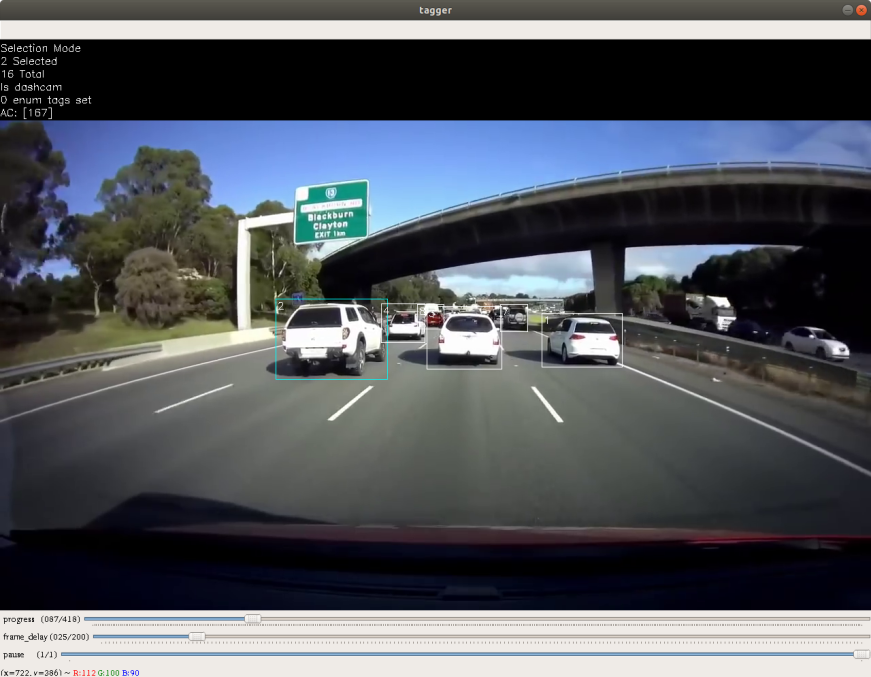
\includegraphics[width=0.5\textwidth]{images/example_gui_tool.png}
		\caption{GUI tool to facilitate annotation}
		\label{fig:example_gui_tool-png}
\end{figure}

%%%%%%%%%%%%%%%%%%%%%%%%%%%%%%%%%%%%%%%%%%%%%%%%%%%%%%%%%%%%%%%%%%%%%%%%%%%%%%%%
\section{EXPERIMENT}
- present results of our data, reference the Kitti dataset and how they presented their own data (histogram of object classes, velocity, acceleration, etc)
- the major contribution we have is the histogram of accident type
- Histogram of data
- Usage of our data (applications) - not a major section, just describe potential in preventing/predicting accidents and their importance


\todo{Write the EXPERIMENT SECTION (analyzing data)}


%%%%%%%%%%%%%%%%%%%%%%%%%%%%%%%%%%%%%%%%%%%%%%%%%%%%%%%%%%%%%%%%%%%%%%%%%%%%%%%%
\section{CONCLUSION}

\todo{Write the conclusion}
A conclusion section is not required. Although a conclusion may review the main points of the paper, do not replicate the abstract as the conclusion. A conclusion might elaborate on the importance of the work or suggest applications and extensions.

%%%%%%%%%%%%%%%%%%%%%%%%%%%%%%%%%%%%%%%%%%%%%%%%%%%%%%%%%%%%%%%%%%%%%%%%%%%%%%%%
\section{FUTURE WORK}

There are many ways that we could improve on our system. This are just a series of ideas that we could think of:
\begin{enumerate}
\item Custom interpolation between input frames: One idea would be to make it easier to modify the method of interpolation between frames. Currently, linear interpolation is always used. Moreover, given a type of interpolation is stored in the metadata, we probably shouldn't store all interpolated frames, rather than just the ones the user has entered. While linear interpolation works great for entering a frame every 10 frames, supporting more interpolations could be great for faster data entry, or even for supporting affine transformations on more complex bounds.

\item Polyhedral bounds: It's always possible to represent a 2-dimensional polyhedron with a matrix $A\in\mathbb{R}^{n\times 2}$, and a vector $b\in\mathbb{R}^2$, given that the polyhedron can be represented by the set $\left\{x\mid Ax\leq b\right\}$. We could use this idea to store masking bounds that can be used for training Mask-RCNN networks in (near-)collision contexts.

\item Web interface: Having a web-based user interface would be advantageous for this project. While currently being used in the context of (near-)collision accident, this software has the potential to become a platform for scraping automation and collaboration. Ideally, people without a technical background would be able to contribute to the microtasking involved, and technical contributors would be in charge of creating and managing the automation and general design of the pipeline.

\end{enumerate}
\todo{Write the future work ideas}

\addtolength{\textheight}{-12cm}

%%%%%%%%%%%%%%%%%%%%%%%%%%%%%%%%%%%%%%%%%%%%%%%%%%%%%%%%%%%%%%%%%%%%%%%%%%%%%%%%

\section*{APPENDIX}

\todo{Write the appendix}

\pgfplotstableread[col sep=comma]{by-classes.csv}\byclass


\begin{figure}[htpb]
		\centering
    \begin{tikzpicture}
    \begin{axis}[
      title={Objects by class},
      xlabel={Class},
      ylabel={Frequency (\# of bounding boxes)},
      xtick=data,
      xticklabels from table={\byclass}{X}
    ]
    \addplot[fill, ybar] table [x expr=\coordindex, y={Y}] \byclass;
    \end{axis}
    \end{tikzpicture}
		\caption{Object by classes in our private database}
		\label{fig:obj-by-class}
\end{figure}


\begin{center}
\begin{tikzpicture}
\begin{axis}[
  title={Example histogram},
  xlabel={Classes},
  ylabel={$\textup{Normal}(\mu=0, \sigma=1)$}
]
\addplot[fill, ybar] table [x=X, y=Y, col sep=comma] {example.csv};
\end{axis}
\end{tikzpicture}
\end{center}


%%%%%%%%%%%%%%%%%%%%%%%%%%%%%%%%%%%%%%%%%%%%%%%%%%%%%%%%%%%%%%%%%%%%%%%%%%%%%%%%

\nocite{*}
\printbibliography

\end{document}
